\documentclass[tikz,border=1mm,10pt]{standalone}
%\usepackage[dvipsnames]{xcolor}
\usepackage{pgfplots}
\pgfplotsset{compat=1.5.1}
\usetikzlibrary{arrows}
\usetikzlibrary{backgrounds}
\begin{document}
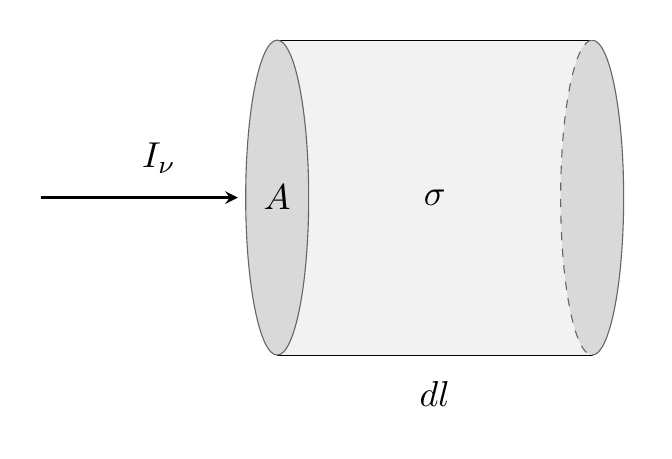
\begin{tikzpicture}[scale=1, transform shape, background rectangle/.style={fill=white}, show background rectangle]


	%main body of cylinder
	\draw[fill=gray!10] (0,0) rectangle (4, 4);

	%draw filled ellipses (surfaces)
	\fill[color=gray!30] (0,2) ellipse (.4 and 2);
	\fill[color=gray!30] (4,2) ellipse (.4 and 2);


	% ellipse edges
	% left ellipse
	\draw[color=darkgray!80] (0, 2) ellipse (.4 and 2);
	% right ellipse
	\begin{scope} % dashed half-ellipse
	\clip (3, 0) rectangle (4, 4);
	\draw[color=darkgray!80, dashed] (4,2) ellipse (.4 and 2);
	\end{scope}
	\begin{scope} % full half-ellipse
	\clip (4, 0) rectangle (4.5, 4);
	\draw[color=darkgray!80] (4, 2) ellipse (.4 and 2);
	\end{scope}


	% Text nodes
	\node[scale=1.3] (a) at (2, -0.5) {$dl$};
	\node[scale=1.3] (a) at (0, 2) {$A$};
	\node[scale=1.3] (b) at (-1.5, 2.5) {$I_{\nu}$};
	\node[scale=1.3] (c) at (2, 2) {$\sigma$};

	% Arrows
	\draw [->, line width = 1 pt, >=stealth] (-3, 2) -- +(2.5,0);
\end{tikzpicture}
\end{document}